% Created 2024-09-18 Wed 17:53
% Intended LaTeX compiler: pdflatex
\documentclass[11pt]{article}
\usepackage[utf8]{inputenc}
\usepackage[T1]{fontenc}
\usepackage{graphicx}
\usepackage{longtable}
\usepackage{wrapfig}
\usepackage{rotating}
\usepackage[normalem]{ulem}
\usepackage{amsmath}
\usepackage{amssymb}
\usepackage{capt-of}
\usepackage{hyperref}
\usepackage{minted}
\usepackage[a4paper, margin=2.5cm]{geometry}
\usepackage{minted}
\usepackage{fontspec}
\setmonofont{Iosevka}
\setminted{fontsize=\small, frame=single, breaklines=true}
\usemintedstyle{emacs}
\usepackage[backend=biber,style=apa]{biblatex}
\addbibresource{citation.bib}
\usepackage{float}
\author{Baley Eccles - 652137 and Tyler Robards - 651790}
\date{\textit{{[}2024-09-12 Thu 14:12]}}
\title{ENG204 - Signals and Linear Systems - Assignment 1.3}
\hypersetup{
 pdfauthor={Baley Eccles - 652137 and Tyler Robards - 651790},
 pdftitle={ENG204 - Signals and Linear Systems - Assignment 1.3},
 pdfkeywords={},
 pdfsubject={},
 pdfcreator={Emacs 29.4 (Org mode 9.8)}, 
 pdflang={English}}
\begin{document}

\maketitle
\tableofcontents

\section{ENG204 - Signals and Linear Systems - Assignment 1.3}
\label{sec:org10174dd}
\subsection{a}
\label{sec:org9f58d4f}
In 1D convolution, the output signal is computed by sliding a filter (also called a kernel) across the input signal, multiplying and summing at each point of overlap. Mathematically, if \(x(t)\) is the input signal and \(h(t)\) is the filter (impulse response), the output signal \(y(t)\) is given by:
\[y(t)=x(t)*h(t)=\int_{-\infty}^{\infty}x(\tau)h(t-\tau)d\tau\]
This process ``blends'' the input signal with the filter, smoothing, sharpening, or otherwise transforming it depending on the characteristics of \(h(t)\). \\
In 2D convolution, we apply the same principles to 2D data, such as images. An image is represented as a matrix of pixel intensities, and the convolution is performed by sliding a 2D kernel (a small matrix) over the image. At each position, the pixel values of the image are multiplied element-wise by the corresponding values of the kernel, and the results are summed to produce the new pixel value in the output image.\\
The 2D convolution of an image \(I(x,y)\) with a filter \(H(u,v)\) is defined as:
\[G(x,y)=I(x,y)*H(u,v)=\sum_u\sum_vI(u,v)H(x-u,y-v)\]
This operation captures how local regions in the image are influenced by the surrounding pixels, which is critical for tasks like edge detection, blurring, and sharpening.\\
In 1D, convolution combines signals by blending neighboring values. In 2D, the same idea is extended to neighboring pixels in both the x- and y-directions, which are weighted by the filter kernel. The kernel can be designed to highlight edges, smooth out noise, or enhance specific features of the image.
\subsection{b}
\label{sec:org2d9b5e1}
\begin{minted}[]{octave}
clear
clc
close

sigma=5;
G = @(x, y) (1/(2*pi*sigma^2)) * exp(-1 * (x.^2 + y.^2) / (2 * sigma^2));
size=ceil(6*sigma);
GFilter=zeros(size);

for xCoord = -size/2:size/2
  for yCoord = -size/2:size/2
    Gval=G(xCoord,yCoord);
    GFilter(size/2+xCoord+1,size/2+yCoord+1)=double(Gval);
  end
end

% Normalise the matrix
GFilter=(GFilter - min(GFilter(:))) / (max(GFilter(:)) - min(GFilter(:)));

\end{minted}


\begin{minted}[]{octave}
noise=imread("/home/Baley/UTAS/ENG204 - Signals And Linear Systems/Assignment 1.3/Pic/image_5_noise.jpg");

output=conv2(noise,GFilter,'same');
imshow(output,[]);

output = output / max(output(:)) * 65535;
imwrite(uint16(output), sprintf('ENG204-Assignment-3-b-sigma-%d.png', sigma));
\end{minted}

\begin{FIGURE}
\begin{figure}[H]
\centering

\includegraphics[width=.9\linewidth]{ENG204-Assignment-3-b-sigma-5.png}
\caption{Image produced with \(\sigma=5\)}
\end{figure}
\end{FIGURE}

\begin{FIGURE}
\begin{figure}[H]
\centering

\includegraphics[width=.9\linewidth]{ENG204-Assignment-3-b-sigma-10.png}
\caption{Image produced with \(\sigma=10\)}
\end{figure}
\end{FIGURE}
From these results we can see that the Gaussian filter blurs the image. When we increase \(\sigma\) the amount of blur increases. This works by replacing the current pixel wiht the average of its surrounding pixels. The pixels at the edges go dark, this is because we are taking the non existant values that are out side the image to be the min value \texttt{(R,G,B)=(0,0,0)} and when we do the convolution we are effectivly bluring the image with black.
\subsection{c}
\label{sec:org22afb3f}
\begin{minted}[]{octave}
clear
clc
close
pkg load symbolic

syms x y p phi sigma
G =(1/(2*pi*sigma)) * exp(-1 * (x^2 + y^2) / (2 * sigma^2));
% Sub in the cylindrical coordinates
xCyl=p*cos(phi);
yCyl=p*sin(phi);
G=subs(G,x,xCyl);
G=subs(G,y,yCyl);
latex(xCyl)
latex(yCyl)
latex(simplify(G))
\end{minted}
To do this we can convert the function to cylindrical coordinates. using:
\[x= \rho \cos{\left(\phi \right)}\]
\[y= \rho \sin{\left(\phi \right)}\]
Which will give:
\[\frac{e^{- \frac{\rho^{2}}{2 \sigma^{2}}}}{2 \pi \sigma}\]
As we can see this does not depend on \(\phi\), which is the rotational aspect, so it is rotationaly symmetric. This means that the filter will be applied equally in all directions.
\subsection{d}
\label{sec:org3fdd75f}
\subsubsection{a}
\label{sec:orgf48f845}
\begin{align*}
G(x,y)&=\frac{1}{2\pi \sigma^{2}}e^{-\frac{x^2+y^2}{2 \sigma^2}} \\
G(x,y)&=\frac{1}{2\pi \sigma^{2}}e^{-\frac{x^2}{2 \sigma^2}}e^{-\frac{y^2}{2 \sigma^2}} \\
\Rightarrow G_x(x)&=\frac{1}{\sqrt{2\pi \sigma^{2}}}e^{-\frac{x^2}{2 \sigma^2}} \\
\textrm{and } G_y(y)&=\frac{1}{\sqrt{2\pi \sigma^{2}}}e^{-\frac{y^2}{2 \sigma^2}}
\end{align*}
This shows that the Guassian kernel can be sperated into two individual components that can be acted separately in the \(x\) and \(y\) directions. We can see that the \(G_x(x)\) and \(G_y(y)\) are varible subsitutions of one another, this means that they will result in the same values given the same input, and hence when formed into their matrices they will be transposes of one another.
\subsubsection{b}
\label{sec:org22ee6ec}
We are taking the convolution of \(G\) and \(I\) resulting in \(O\):
\begin{align*}
O&=I*G                     \\
O&=I*(G_x\cdot G_y)        \\
I'&=I*G_x                  \\
O&=I'* G_y                 \\
O&=(I*G_x)*G_y
\end{align*}
This shows that the Guassian kernel can be convoluted with the image in the \(x\) direction to get some intermediate image, which then can be convoluted in the \(y\) direction to get the final image.
\subsubsection{c}
\label{sec:org42444d1}
\begin{minted}[]{octave}
clear
clc
close
sigma=10;
size=ceil(6*sigma);



noise=imread("/home/Baley/UTAS/ENG204 - Signals And Linear Systems/Assignment 1.3/Pic/image_5_noise.jpg");

tic
G = @(x, y) (1/(2*pi*sigma^2)) * exp(-1 * (x.^2 + y.^2) / (2 * sigma^2));
GFilter=zeros(size);
for xCoord = -size/2:size/2
  for yCoord = -size/2:size/2
    Gval=G(xCoord,yCoord);
    GFilter(size/2+xCoord+1,size/2+yCoord+1)=double(Gval);
  end
end
GFilter=(GFilter - min(GFilter(:))) / (max(GFilter(:)) - min(GFilter(:)));
single=conv2(noise,GFilter,'same');
time1 = toc;

tic
Gx = @(x) (1/(sqrt(2*pi*sigma^2))) * exp(-1 * (x.^2) / (2 * sigma^2));
Gy = @(y) (1/(sqrt(2*pi*sigma^2))) * exp(-1 * (y.^2) / (2 * sigma^2));
GxFilter=zeros(size,1);
GyFilter=zeros(1,size);
for xCoord = -size/2:size/2
  Gxval=Gx(xCoord);
  GxFilter(size/2+xCoord+1,1)=double(Gxval);
end
for yCoord = -size/2:size/2
  Gyval=Gy(yCoord);
  GyFilter(1,size/2+yCoord+1)=double(Gyval);
end
GxFilter=(GxFilter - min(GxFilter(:))) / (max(GxFilter(:)) - min(GxFilter(:)));
GyFilter=(GyFilter - min(GyFilter(:))) / (max(GyFilter(:)) - min(GyFilter(:)));
output=conv2(noise,GxFilter,'same');
double=conv2(output,GyFilter,'same');
time2 = toc;


subplot(2, 1, 1);
imshow(single, []);

title('single');
subplot(2, 1, 2);
imshow(double, []);

title('double');
fprintf('The time to calculate the convolution of the single matrix is %f s\n', time1);
fprintf('The time to calculate the convolution of the two matrices is %f s\n', time2);


% sacle them so they dont look weird
single = single / max(single(:)) * 65535;
double = double / max(double(:)) * 65535;
% Save the images
imwrite(uint16(single), 'ENG204-Assignment-3-Single-sigma-10.png');
imwrite(uint16(double), 'ENG204-Assignment-3-Double-sigma-10.png');
\end{minted}

The output with \(\sigma=10\) is:
\begin{itemize}
\item The time to calculate the convolution of the single matrix is 0.430982 s
\item The time to calculate the convolution of the two matrices is 0.100643 s
\end{itemize}
As we can see the convolution of the two matrices is about four times as fast. And we can also see that this creates the exact same result.\\
\begin{FIGURE}
\begin{figure}[H]
\centering

\includegraphics[width=.9\linewidth]{ENG204-Assignment-3-Single-sigma-10.png}
\caption{Image with one convolution}
\end{figure}
\end{FIGURE}
\begin{FIGURE}
\begin{figure}[H]
\centering

\includegraphics[width=.9\linewidth]{ENG204-Assignment-3-Double-sigma-10.png}
\caption{Image with two convolution}
\end{figure}
\end{FIGURE}
Increasing the \(\sigma\) we will see that the difference between the two times increases. For \(\sigma=50\):
\begin{itemize}
\item The time to calculate the convolution of the single matrix is 6.112394 s
\item The time to calculate the convolution of the two matrices is 0.139590 s
\end{itemize}
Here we get a \(\approx 50\) times increase in speed. These results will vary based upon the hardware that it is being run on. However, we would still expect to see the increase in speed from one convolution to two.\\
We can also notice that the increase in time between each \(\sigma\) grows faster for the single convolution compared to the double convolution. That is, for the single convolution, from \(\sigma=10\) to \(\sigma=50\), we get a \(\approx 14\) times time requirement, and for the double convolution we \(\approx 1.4\) times time requirement. This shows that not only does the double convolution perform better than the single convolution, but it also grows slower when \(\sigma\) increases. So, it is better to calculate the one dimentional matrix than the two dimentional ones. This could also be improved by using the transpose property discussed in \hyperref[sec:orgf48f845]{a}, this would eliminate the need to calculate the second matrix.
\subsection{e}
\label{sec:orgd16ab25}
\begin{align*}
\nabla^{2}f &= \frac{\partial^2 f}{\partial x^2}+ \frac{\partial^2 f}{\partial y^2} \\
\textrm{subsitute in } \frac{\partial^2 f}{\partial x^2} &\approx f(x+1,y)-2f(x,y)+f(x-1,y) \\
\textrm{and } \frac{\partial^2 f}{\partial y^2} &\approx f(x,y+1)-2f(x,y)+f(x,y-1) \\
\textrm{gives }\nabla^{2}f & \approx \left[ f(x+1,y) + f(x-1,y) + f(x,y+1) + f(x,y-1)\right] - 4f(x,y)
\end{align*}

Reading the coefficents for the matrix:
\[L=\begin{bmatrix}
0 & 1  & 0 \\
1 & -4 & 1 \\
0 & 1  & 0
\end{bmatrix}\]
\subsection{f}
\label{sec:org18e8365}
\begin{minted}[]{octave}
clear
clc
close

LFilter=[0, 1, 0;
         1,-4, 1;
         0, 1, 0];

\end{minted}

\begin{minted}[]{octave}
noise=imread("/home/Baley/UTAS/ENG204 - Signals And Linear Systems/Assignment 1.3/Pic/image_5_noise.jpg");

noise = double(noise);
noise = uint8(255 * (noise - min(noise(:))) / (max(noise(:)) - min(noise(:))));
output=conv2(noise,LFilter,'same');
Threshold = 25;
EdgeDetect = output < Threshold;
imshow(EdgeDetect,[]);

EdgeDetect = EdgeDetect / max(EdgeDetect(:)) * 65535;
imwrite(uint16(EdgeDetect), 'ENG204-Assignment-3-f-1.png');
\end{minted}
Noise in the image makes the derivative of the image contain a lot of larger values. The noise makes the difference between each pixel a larger result than without the noise. This results in the edge detect image having a lot of large values, requiring the threshold to be larger and reducing the amount of true edges being detected.
\begin{FIGURE}
\begin{figure}[H]
\centering
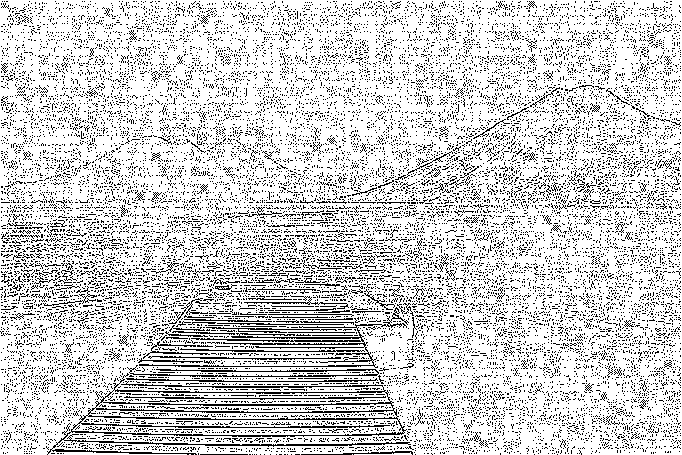
\includegraphics[width=.9\linewidth]{ENG204-Assignment-3-f-1.png}
\caption{Edge detect image}
\end{figure}
\end{FIGURE}
\subsection{g}
\label{sec:orga915e23}

\begin{align*}
LoG(x,y) &= \nabla^2G(x,y) = \frac{\partial^2 G}{\partial x^2} + \frac{\partial^2 G}{\partial y^2}\\
&\\
\frac{\partial G}{\partial x}&=- \frac{x e^{-\frac{ x^{2} + y^2}{2 \sigma^{2}}}}{2 \pi \sigma^{3}} \\
\Rightarrow \frac{\partial^2 G}{\partial x^2}&=- \frac{e^{-\frac{ x^{2} + y^2}{2 \sigma^{2}}}}{2 \pi \sigma^{3}} + \frac{x^{2} e^{-\frac{ x^{2} + y^2}{2 \sigma^{2}}}}{2 \pi \sigma^{5}} \\
& \\
\frac{\partial G}{\partial y}&=-\frac{y e^{-\frac{ x^{2} + y^2}{2 \sigma^{2}}}}{2 \pi \sigma^{4}}\\
\Rightarrow \frac{\partial^2 G}{\partial y^2}&=-\frac{e^{-\frac{ x^{2} + y^2}{2 \sigma^{2}}}}{2 \pi \sigma^{4}} + \frac{y^{2} e^{-\frac{ x^{2} + y^2}{2 \sigma^{2}}}}{2 \pi \sigma^{6}}
& \\
\Rightarrow LoG(x,y) &=- \frac{e^{-\frac{ x^{2} + y^2}{2 \sigma^{2}}}}{\pi \sigma^{4}} + \frac{x^{2} e^{-\frac{ x^{2} + y^2}{2 \sigma^{2}}}}{2 \pi \sigma^{6}} + \frac{y^{2} e^{-\frac{ x^{2} + y^2}{2 \sigma^{2}}}}{2 \pi \sigma^{6}}\\
\Rightarrow LoG(x,y) &=-\frac{1}{\pi\sigma^4}\left(1-\frac{x^2+y^2}{2\sigma^2}\right)e^{-\frac{x^2+y^2}{2\sigma^{2}}}
\end{align*}
\subsection{h}
\label{sec:org1105e8e}
Focusing on \(1-\frac{x^2+y^2}{2\sigma^2}\) in the kernel. We can see that it contains \(x^2+y^2\), which is not separable, so the entire kernel is not separable. \\
The second derivative of the Gaussian kernel can be expressed as a product of an individual variable and the Gaussian kernel. That is:
\begin{align*}
\frac{\partial^2 G}{\partial x^2}&=-\frac{e^{-\frac{ x^{2} + y^2}{2 \sigma^{2}}}}{2 \pi \sigma^{3}} + \frac{x^{2} e^{-\frac{ x^{2} + y^2}{2 \sigma^{2}}}}{2 \pi \sigma^{5}} \\
\frac{\partial^2 G}{\partial x^2}&=\frac{1}{2\pi\sigma^2}e^{-\frac{x^2+y^2}{2\sigma^2}} \left( \frac{x^2}{\sigma^3}-\frac{1}{\sigma}\right) \\
\frac{\partial^2 G}{\partial x^2}&=G(x,y)\left( \frac{x^2}{\sigma^3}-\frac{1}{\sigma}\right) \\
& \\
& \textrm{Similarly for } \frac{\partial^2 G}{\partial y^2}\\
\frac{\partial^2 G}{\partial y^2}&=\frac{1}{2\pi\sigma^2}e^{-\frac{y^2+x^2}{2\sigma^2}} \left( \frac{y^2}{\sigma^3}-\frac{1}{\sigma}\right) \\
\frac{\partial^2 G}{\partial y^2}&=G(x,y)\left( \frac{y^2}{\sigma^3}-\frac{1}{\sigma}\right)
\end{align*}
We know that the Gaussian kernel is separable, and that is being multiplied by a function of the respective variable. So, the derivatives of the Guassian kernel are separable.\\
To speed up the computation of the LoG kernel, we can use:
\[\nabla^2 G\approx \frac{\partial^2 G}{\partial x^2} + \frac{\partial^2 G}{\partial y^2}\]
Where we can calculate the first and second derivatives from their separable forms.
\subsection{i}
\label{sec:orgea963d5}
\begin{minted}[]{octave}
clear
clc
close

sigma=2;

LoG = @(x, y) (-1/(pi*sigma^4))*(1- ((x.^2+y.^2)/(2*sigma^2)))*e^(-1*(x^2+y^2)/(2*sigma^2));
size=ceil(6*sigma);
LoGFilter=zeros(size);

for xCoord = -size/2:size/2
  for yCoord = -size/2:size/2
    LoGval=LoG(xCoord,yCoord);
    LoGFilter(size/2+xCoord+1,size/2+yCoord+1)=double(LoGval);
  end
end


\end{minted}


\begin{minted}[]{octave}
close
noise=imread("/home/Baley/UTAS/ENG204 - Signals And Linear Systems/Assignment 1.3/Pic/image_5_noise.jpg");
noise = double(noise);
noise = uint8(255 * (noise - min(noise(:))) / (max(noise(:)) - min(noise(:))));
output=conv2(noise,LoGFilter,'same');
imshow(output,[]);
output = double(output);
output = uint8(255 * (output - min(output(:))) / (max(output(:)) - min(output(:))));
Threshold = 120;
EdgeDetect = output < Threshold;
subplot(1, 2, 1);
imshow(output,[]);
title('LoG');
subplot(1, 2, 2);
imshow(EdgeDetect,[]);
title('Edge Detect');

imwrite(EdgeDetect, sprintf('ENG204-Assignment-3-i-EdgeDetect-sigma-%d.png', sigma));
imwrite(output, 'ENG204-Assignment-3-i-LoG.png');
\end{minted}
\begin{FIGURE}
\begin{figure}[H]
\centering
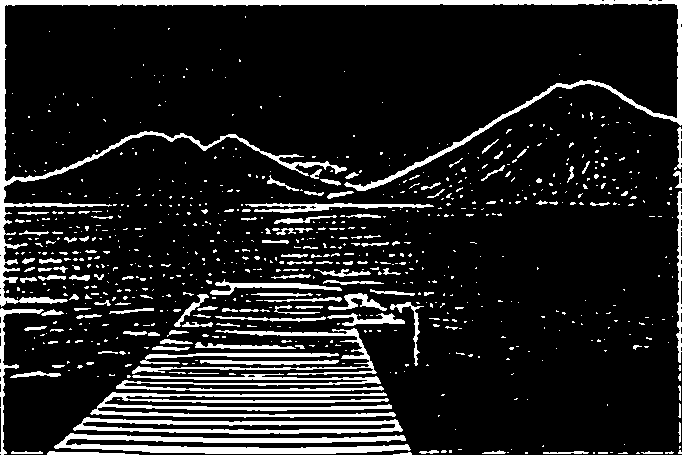
\includegraphics[width=.9\linewidth]{ENG204-Assignment-3-i-EdgeDetect-sigma-2.png}
\caption{The new edge detect image}
\end{figure}
\end{FIGURE}
Comparing this to the other edge detect image, we notice that there are a lot fewer artifacts in the sky. When the standard deviation is increased, it could be seen that the edges of the objects became larger and less sensitive to noise and small edges.
\subsection{j}
\label{sec:org416e70f}
To sharpen the image, we will get an edge detection of the image and then take it away from the original image. However, as mentioned before, the noise in the image will make it look bad, so first we are going to apply the Gaussian filter and then the edge detection.
\begin{minted}[]{octave}
clear
clc
close

sigma=3;
size=ceil(6*sigma);
Gx = @(x) (1/(sqrt(2*pi*sigma^2))) * exp(-1 * (x.^2) / (2 * sigma^2));
Gy = @(y) (1/(sqrt(2*pi*sigma^2))) * exp(-1 * (y.^2) / (2 * sigma^2));
GxFilter=zeros(size,1);
GyFilter=zeros(1,size);
for xCoord = -size/2:size/2
  Gxval=Gx(xCoord);
  GxFilter(size/2+xCoord+1,1)=double(Gxval);
end
for yCoord = -size/2:size/2
  Gyval=Gy(yCoord);
  GyFilter(1,size/2+yCoord+1)=double(Gyval);
end
GxFilter=(GxFilter - min(GxFilter(:))) / (max(GxFilter(:)) - min(GxFilter(:)));
GyFilter=(GyFilter - min(GyFilter(:))) / (max(GyFilter(:)) - min(GyFilter(:)));

LFilter=[0, 1, 0;
         1,-4, 1;
         0, 1, 0];
\end{minted}


\begin{minted}[]{octave}
close
noise=imread("/home/Baley/UTAS/ENG204 - Signals And Linear Systems/Assignment 1.3/Pic/image_5_noise.jpg");
noise = double(noise);
noise = uint8(255 * (noise - min(noise(:))) / (max(noise(:)) - min(noise(:))));

Blur1=conv2(noise,GxFilter,'same');
Blur=conv2(Blur1,GyFilter,'same');

Edge=conv2(Blur,LFilter,'same');

output=noise-2*Edge;

subplot(1, 4, 1);
imshow(output, []);
title('Sharpened');
subplot(1, 4, 2);
imshow(Edge, []);
title('Edge');
subplot(1, 4, 3);
imshow(Blur, []);
title('Blur');
subplot(1, 4, 4);
imshow(noise, []);
title('Original');

imwrite(output, 'ENG204-Assignment-3-Sharpened.png');
imwrite(Edge, 'ENG204-Assignment-3-Edge.png');
imwrite(Blur, 'ENG204-Assignment-3-Blur.png');
imwrite(noise, 'ENG204-Assignment-3-Original.png');

\end{minted}

\begin{FIGURE}
\begin{figure}[H]
\centering
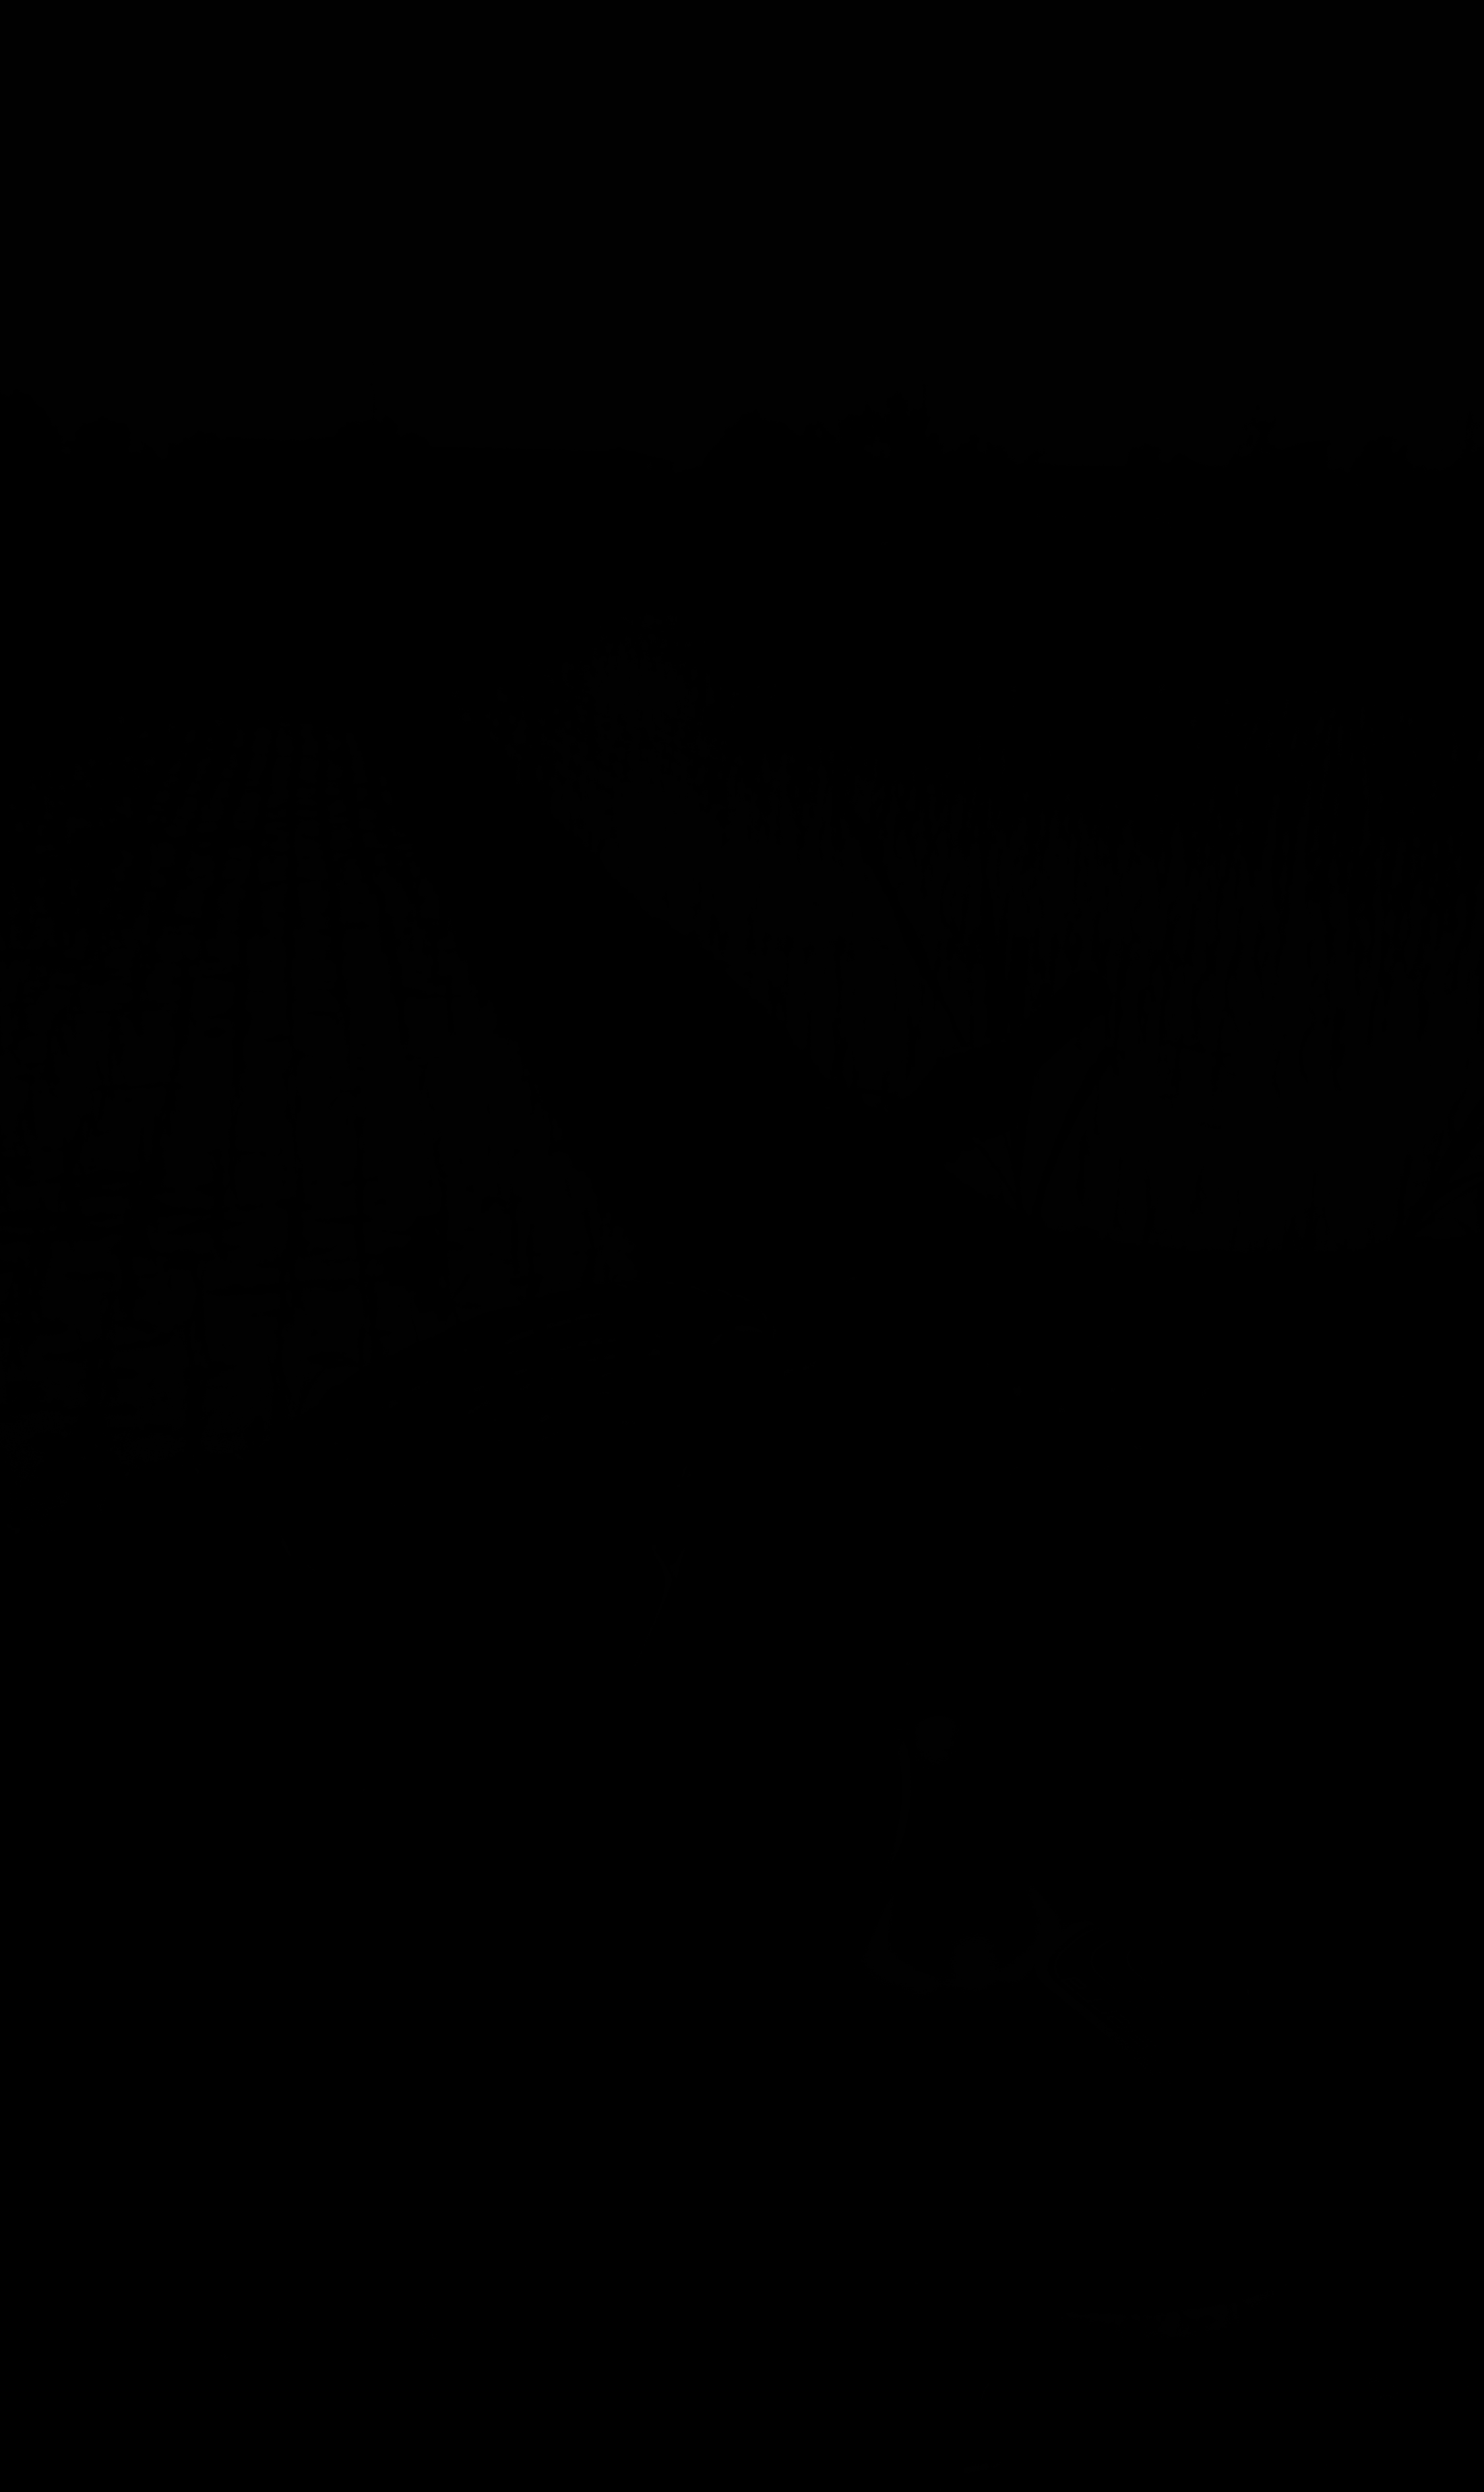
\includegraphics[width=.9\linewidth]{ENG204-Assignment-3-Original.png}
\caption{Original image}
\end{figure}
\end{FIGURE}
\begin{FIGURE}
\begin{figure}[H]
\centering
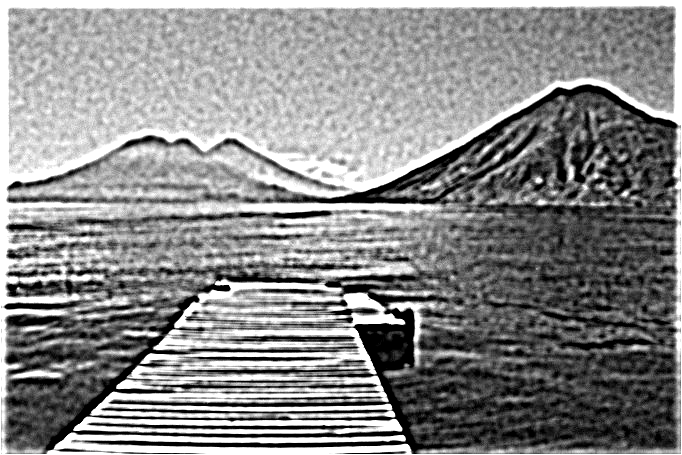
\includegraphics[width=.9\linewidth]{ENG204-Assignment-3-Sharpened.png}
\caption{Image sharpened a lot to exagerate the effects}
\end{figure}
\end{FIGURE}
From this result, we can see that it highlights the edges of the mountains and dock.
\end{document}
